\documentclass[12pt,letterpaper]{article}

% --- Paquetes Requeridos ---
\usepackage[utf8]{inputenc}
\usepackage[spanish,es-tabla]{babel}
\usepackage[margin=2.5cm]{geometry}
\usepackage{graphicx}
\usepackage{float}
\usepackage{titlesec}
\usepackage{setspace}
\usepackage{hyperref}
\usepackage{booktabs}
\usepackage{caption}
\usepackage{enumitem}
\usepackage{listings}
\usepackage{xcolor}

% --- Configuración de Párrafo ---
\onehalfspacing
\setlength{\parindent}{0pt}
\setlength{\parskip}{1em}

% --- Rutas de búsqueda de imágenes ---
% Permite compilar tanto desde Documentos/Entregables/ como con todas las
% imágenes en una sola carpeta plana.
\graphicspath{{./}{../Evidencia/}{Evidencia/}{imagenes/}}

% --- Configuración de listings ---
\lstset{
    basicstyle=\ttfamily\footnotesize,
    breaklines=true,
    frame=single,
    captionpos=b,
    showstringspaces=false
}

% --- Inicio del Documento ---
\begin{document}

% --- PORTADA ---
\begin{titlepage}
    \centering

    {\Large \textbf{UNIVERSIDAD SANTO TOMÁS}} \\[1cm]

    {\Large \textbf{Sistema colaborativo de robots móviles para asistencia de orientación en entornos interiores con múltiples pisos}} \\[2cm]

    {\large \textbf{Realizado por:}} \\
    {\large Santiago Hernández Ávila} \\
    {\large Jonny Alejandro Mejía León} \\[1cm]

    \begin{figure}[H]
        \centering
        \includegraphics[width=0.6\textwidth]{Logos Uni.png}
        \label{Logo Universidad Santo Tomas y facultad de ingenieria electronica}
    \end{figure}

    \vfill

    {\large \textbf{Informe de Avance --- Semana 26}} \\
    {\large Fase 5: integración del sistema y realización de pruebas} \\
    {\large Navegación de un vehículo y sistema completo con los dos vehículos} \\[1.5cm]

    \textbf{Dirigido por:} \\
    Ing. Armando Mateus Rojas, Msc. \\
    Ing. Nestor Ivan Ospina, Msc. \\
    Ing. Oscar Mauricio Gélvez Lizarazo, Msc. \\[1.0cm]

    \vfill

    {\large GED (Grupo de Estudio y Desarrollo en Robótica)} \\
    {\large Facultad de Ingeniería Electrónica} \\
    {\large División de Ingenierías} \\
    {\large Bogotá, octubre de 2026}
\end{titlepage}

% --- CONTENIDO ---

\section{Introducción}

Este informe presenta el avance de la semana 26 del cronograma (5 al 9 de octubre de 2026, con corte el viernes 9), dentro de la fase 5, integración del sistema y realización de pruebas.

La semana tenía dos metas: alcanzar la compuerta G-3, la navegación de un vehículo con la llegada verificada, y correr la primera misión con relevo entre los dos vehículos, la compuerta G-5. El relevo es el traspaso del usuario del vehículo de un piso al vehículo del otro. Las compuertas son las condiciones verificables que el acta de la decisión GO/NO-GO fija para continuar con la demostración física, cada una con la fecha de su corte~\cite{acta}.

G-3 se alcanzó el 7 de octubre, después de integrar en los dos vehículos la unidad de medición inercial (IMU) de su tarjeta. G-5 no se corrió: el 8 de octubre, con los dos vehículos navegando a la vez, sus tarjetas se saturaron. El coordinador, el programa que asigna las misiones y organiza el relevo, pasó el 9 de octubre de un vehículo al computador portátil, y esa noche el sistema completo se probó en el laboratorio con los dos vehículos. La Tabla~\ref{tab:compuertas} resume el estado de las compuertas.

\begin{table}[H]
    \centering
    \small
    \caption{Compuertas del acta GO/NO-GO al 9 de octubre.}
    \label{tab:compuertas}
    \begin{tabular}{@{}p{3.4cm}p{6.6cm}p{4.0cm}@{}}
        \toprule
        \textbf{Compuerta} & \textbf{Qué exige} & \textbf{Estado al 9 de octubre} \\ \midrule
        G-1, actuación & El vehículo responde a las órdenes de dirección y tracción & Alcanzada el 22 de septiembre \\ \addlinespace
        G-2, odometría & Error de la odometría, la estimación del desplazamiento del vehículo, de hasta 10~\% sobre un recorrido medido de al menos 5~m & Alcanzada el 2 de octubre \\ \addlinespace
        G-3, navegación de un vehículo & Un recorrido de punto a punto con Nav2, el sistema de navegación de ROS~2, con la llegada verificada & Alcanzada el 7 de octubre \\ \addlinespace
        G-4, coexistencia & Los dos vehículos y el coordinador en la misma red, sin conflicto de nombres & Alcanzada el 22 de septiembre \\ \addlinespace
        G-5, protocolo completo & Una misión (guiar a un usuario de un origen a un destino) con relevo entre los dos vehículos, uno en cada piso & Pendiente \\ \addlinespace
        G-6, RF-27 & Las repeticiones de RF-27, el requisito de la campaña física, con el protocolo completo & Pendiente; requiere G-5 \\ \bottomrule
    \end{tabular}
\end{table}

\section{Objetivos de la semana}

El cronograma fija para esta semana el siguiente criterio de cierre~\cite{cronograma}:

\begin{quote}
\textit{Gráficas y tablas de las cuatro métricas; tabla de cumplimiento requisito por requisito.}
\end{quote}

El criterio no se cumplió. El 25 de septiembre, al replanificar contra las fechas del acta, la misión con relevo (G-5) pasó a esta semana y la campaña de RF-27 a la semana 27; sin ellas no hay métricas físicas que graficar. La semana se organizó en \texttt{PLAN\_S26.md}~\cite{plan}: la IMU, la red entre los dos pisos, G-3, la media vuelta del vehículo y G-5. Se cumplió todo salvo G-5.

\section{Resolución de los directores del 5 de octubre}

Los autores consultaron a los directores sobre el cambio de sitio, el corte C-1 y el regreso automático del vehículo después de una misión. Los acuerdos, verbales, quedaron en la sección 6.2 del acta~\cite{acta}:

\begin{enumerate}[leftmargin=*]
    \item Se acepta el cambio de sitio a los pasillos de los pisos 3 y 4 del edificio, que los directores trataron también con los evaluadores.
    \item Sobre el corte C-1, la indicación fue organizar el trabajo para presentar a tiempo, sin una fecha nueva. Los autores la aplican así: la demostración con los vehículos continúa, G-3 sigue abierta con su tolerancia de 0,5~m y los cortes C-2 (9 de octubre) y C-3 (16 de octubre) se mantienen.
    \item El vehículo vuelve a su punto de partida solo cuando el usuario cancela una misión (requisito RF-29). Entre misiones no vuelve: cada misión empieza donde terminó la anterior, y las pruebas de G-5 y G-6 se hacen sin reubicar los vehículos a mano.
\end{enumerate}

\section{Unidad de medición inercial en los dos vehículos}

Hasta esta semana el vehículo estimaba su movimiento solo con el LiDAR, el sensor láser que mide las distancias alrededor, mediante rf2o, un paquete que calcula el desplazamiento comparando barridos consecutivos. El 5 de octubre se comprobó que la tarjeta de los dos vehículos incluye una IMU (un giroscopio y un acelerómetro), una Bosch BMI160~\cite{imu}. En los dos, el giroscopio midió giros de 90$^\circ$ y 360$^\circ$ hechos a mano con un error de 0,1~\% a 1,3~\%, y quieto no se desvió más de 0,3$^\circ$ en 60~s. Solo un criterio no se cumplió: la aceleración en reposo de \texttt{amss-jgm9}, 10,268~m/s$^2$ frente a un límite de 10,11~m/s$^2$, un desfase del acelerómetro que no afecta al giroscopio.

La IMU se integró en la navegación con un filtro de Kalman extendido (EKF), que toma de rf2o el avance y de la IMU el giro~\cite{integracion}. En un giro de 90$^\circ$ hecho a mano contra una línea del piso, el filtro midió +90,17$^\circ$ en \texttt{amss-jgm9} y +88,38$^\circ$ en \texttt{amss-ez9n}. Con el vehículo quieto, el rumbo del filtro se movió 0,3$^\circ$ o menos por minuto; rf2o solo derivó hasta 5,9$^\circ$ por minuto. Para no sobrecargar la tarjeta, la IMU publica a 25~Hz y el filtro corre a 15~Hz.

\section{Red inalámbrica entre los dos pisos}

Jonny Mejía montó la red del sitio nuevo, con un punto de acceso por piso. El 5 de octubre encontró que los dos vehículos no podían transmitir en la banda de 5~GHz~\cite{red5}. A su sistema le faltaba la base de datos de reglas de radio por país, y sin ella las 31 frecuencias de esa banda quedaban solo para escuchar. Instalada la base, los dos pasaron a 13 canales utilizables. El requisito RF-15 (latencia acotada entre los vehículos y el coordinador) se midió de nuevo entre los dos vehículos sobre 5~GHz y cumple. La latencia mediana fue de 5,99~ms y el percentil 95 de 11,12~ms, frente a 7,61~ms y 20,76~ms en septiembre.

El 7 de octubre se encontró un bucle en la red~\cite{bucle}. Un punto de acceso conectado a la vez por cable y por su enlace inalámbrico de malla entregaba cada paquete hasta tres veces: 147 paquetes recibidos por cada 100 enviados. Con el enlace de malla apagado, la latencia entre los dos vehículos quedó en 3,75~ms de promedio, con 0,51~ms de variación.

\section{Navegación encadenada en el piso 4 y compuerta G-3}
\label{sec:piso4}

El 7 de octubre el vehículo \texttt{amss-jgm9} recorrió en el piso 4 tres tramos encadenados, de la salida a los salones 403, 402 y 401, sin que nadie lo tocara, y después regresó a la salida~\cite{piso4}. Navegó con Nav2 y AMCL, el método de localización sobre el mapa, con la IMU integrada y el margen de llegada de Nav2 reducido de 1,0~m a 0,5~m (Tabla~\ref{tab:piso4}).

\begin{table}[H]
    \centering
    \small
    \caption{Llegadas de la cadena del piso 4 del 7 de octubre.}
    \label{tab:piso4}
    \begin{tabular}{@{}p{3.6cm}p{3.2cm}p{7.0cm}@{}}
        \toprule
        \textbf{Llegada} & \textbf{Distancia a la meta} & \textbf{Cómo se obtuvo} \\ \midrule
        Salón 403 & 0,26~m & Estimada con el error de los otros tramos; no se midió \\
        Salón 402 & 0,45~m & Flexómetro, de marca a marca \\
        Salón 401 & 0,06~m & Flexómetro, de marca a marca \\
        Regreso a la salida & 0,34~m & Flexómetro, contra las paredes \\ \bottomrule
    \end{tabular}
\end{table}

Las llegadas quedaron dentro de la tolerancia de 0,5~m, y G-3 se declaró alcanzada en el acta. El 2 de octubre, sin IMU y con margen de 1,0~m, habían quedado a 0,57~m y 0,62~m. La odometría del filtro sobreestimó el avance un 1,9~\% y un 4,9~\% en los dos tramos medidos, dentro del 10~\% de G-2. La escala de velocidad de \texttt{amss-jgm9} quedó en 0,9: con 1,0 iba a 1,36~m/s y se pasaba de la meta unos 0,7~m.

\begin{figure}[H]
    \centering
    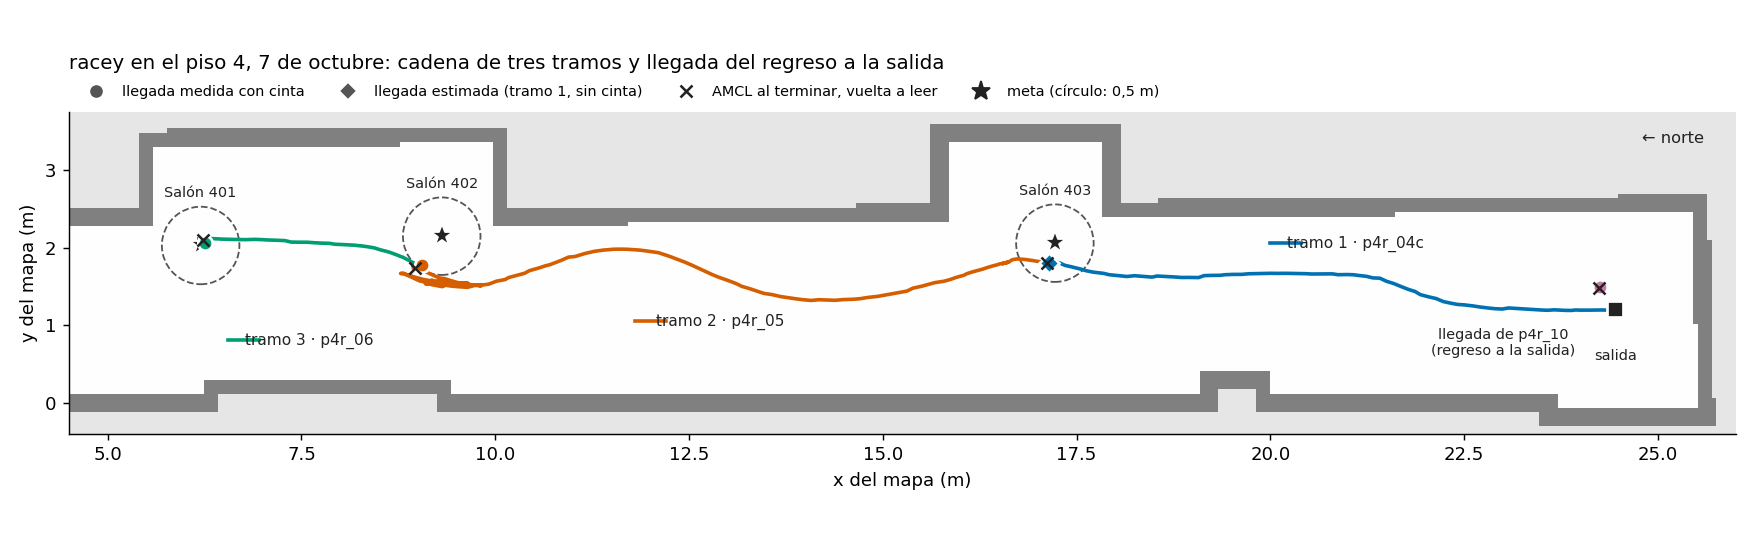
\includegraphics[width=\textwidth]{S26_piso4_cadena_racey.png}
    \caption{Cadena de tres tramos de \texttt{amss-jgm9} en el piso 4 y regreso a la salida: recorrido según AMCL, llegadas medidas con flexómetro, la llegada estimada al Salón 403 y la posición de AMCL al terminar cada tramo.}
    \label{fig:cadena}
\end{figure}

\section{Media vuelta para ir a recoger al usuario}

Entre misiones el vehículo sale desde donde terminó la anterior (sección 3), y a veces el siguiente origen queda detrás. Con dirección de tipo Ackermann, como la de un automóvil, el vehículo no puede girar sobre sí mismo, y en pasillos de 2,3 a 3,2~m de ancho tiene que dar la vuelta en varios tiempos.

El 7 de octubre la media vuelta con Nav2 abortó dos veces contra la pared en la salida del piso 4, de 2,5~m de ancho~\cite{piso4}. Con la misma orden de velocidad, el motor retrocedía a unas 1,7 veces la velocidad con que avanzaba. Por eso se agregó al programa que traduce las órdenes al motor una escala para la marcha atrás, fijada en 0,75 en los dos vehículos. La media vuelta en dos tiempos, marcha atrás con la dirección a tope y avance con la dirección contraria, giró 182$^\circ$, y después Nav2 llegó al Salón 403 en 18,7~s (Figura~\ref{fig:mediavuelta}).

\begin{figure}[H]
    \centering
    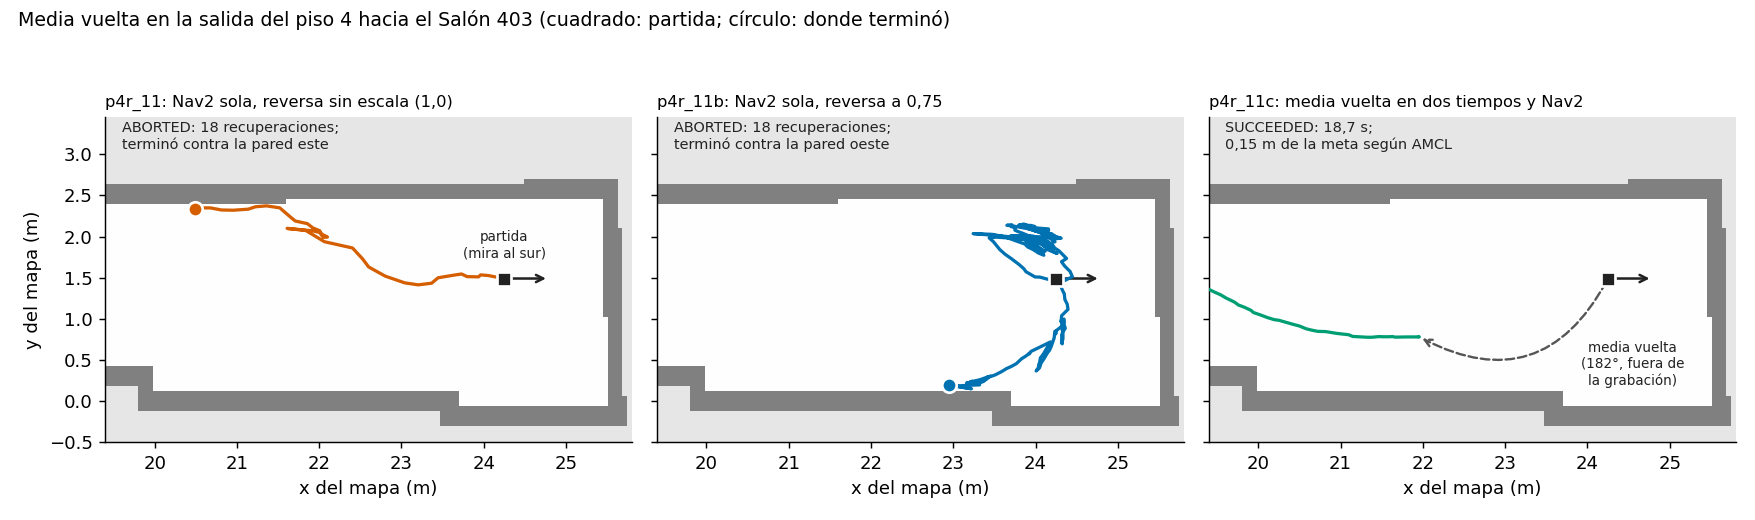
\includegraphics[width=0.85\textwidth]{S26_piso4_media_vuelta.png}
    \caption{Trayectorias de los tres intentos de media vuelta en la salida del piso 4: los dos de Nav2, que abortaron, y el de dos tiempos, que giró 182$^\circ$.}
    \label{fig:mediavuelta}
\end{figure}

Esa maniobra se incorporó al agente, el programa que corre en cada vehículo. Alterna marcha atrás y avance y corta cada tiempo cuando la huella prevista del vehículo queda a menos de 0,10~m de un obstáculo, visto con el LiDAR o marcado en el mapa. El LiDAR no detecta el borde de una escalera, así que en el mapa la escalera está cerrada. El coordinador la pide antes de una meta que queda detrás del vehículo. El 8 de octubre se probó en \texttt{amss-ez9n}: giró 160$^\circ$ frente al Salón 301 y 167$^\circ$ junto a la escalera, alejándose de ella~\cite{estado}.

\section{Navegación en el piso 3}

El 8 de octubre \texttt{amss-ez9n} recorrió el piso 3 en cuatro tramos sin que nadie lo tocara: de la salida a los salones 303, 302 y 301, y de vuelta a la escalera~\cite{estado}. Los cuatro terminaron con éxito y sin recuperaciones de Nav2, con llegadas a entre 0,10~m y 0,27~m de la meta según AMCL. Estas llegadas no se midieron con flexómetro.

\section{Carga de las tarjetas y coordinador en el portátil}

El 8 de octubre se intentó G-5 con los dos vehículos navegando a la vez y el coordinador en \texttt{amss-jgm9}~\cite{estado}. La tarjeta de ese vehículo llegó a una carga de 22 a 33, sobre dos núcleos, y Nav2 abortaba al arrancar. La causa era el descubrimiento de ROS~2, el mecanismo con que los programas se encuentran en la red. Con los dos vehículos, unos cuarenta programas se anunciaban a todos los demás por la red inalámbrica, a unos 2000 paquetes por segundo. Con el descubrimiento limitado al interior de cada vehículo, la carga bajó a 1,6 y el tráfico a unos 600 paquetes por segundo, pero el coordinador dejó de ver la navegación del otro vehículo.

El 9 de octubre el coordinador y el grabador de las misiones pasaron al portátil, que es el servidor central del diseño. El portátil tiene ROS~2 Humble y los vehículos ROS~2 Jazzy, cuyas acciones de navegación no son compatibles. Por eso el coordinador corre en un contenedor: un entorno aislado del portátil con su propia versión de ROS, en este caso Jazzy. Cada vehículo tiene al portátil como único equipo conocido, y los vehículos no se comunican entre sí.

Esa noche se probó el sistema completo en el laboratorio con los dos vehículos, con las ruedas en el aire para las pruebas de navegación~\cite{laboratorio}. El portátil vio la navegación y el estado de los dos. La página de la interfaz se abrió desde un teléfono y las misiones pedidas desde allí llegaron al coordinador. La carga de las tarjetas, con todo el sistema en marcha, se resume en la Tabla~\ref{tab:carga}.

\begin{table}[H]
    \centering
    \small
    \caption{Carga de las tarjetas con el sistema completo, en el laboratorio, el 9 de octubre.}
    \label{tab:carga}
    \begin{tabular}{@{}p{6.6cm}p{3.6cm}p{3.6cm}@{}}
        \toprule
        & \texttt{amss-ez9n} & \texttt{amss-jgm9} \\ \midrule
        Procesador de la tarjeta, en reposo & 54~\% & 59~\% \\
        Procesador de la tarjeta, navegando & 68~\% (máximo 72~\%) & 74~\% (máximo 79~\%) \\
        Veces que el controlador de Nav2 no alcanzó sus 10~Hz & 1 en 76~s & 5 en 146~s \\
        Frecuencia mínima del controlador & 5,8~Hz & 5,5~Hz \\ \bottomrule
    \end{tabular}
\end{table}

Con los datos de esa sesión se hicieron tres ajustes. El planificador de Nav2 calcula al arrancar una tabla de distancias alrededor del vehículo. Con 10~m en lugar de 20~m, ese cálculo pasó de 81~s a entre 19~s y 23~s. La ruta más larga del piso 4, de unos 18~m, se calculó en 0,31~s, dentro del plazo de 2~s. Además, rf2o dejó de escribir sus mensajes informativos, que ocupaban casi todo el registro y le costaban al programa de arranque un 3,5~\% de un núcleo. El guion de arranque espera ahora a que Nav2 esté activo, en lugar de un tiempo fijo. Las dos cadenas quedan listas en 4~min 4~s y 4~min 22~s, frente a 4~min 45~s con el planificador todavía sin activar.

\section{Simulación tras la actualización de ROS}

El 6 de octubre, en el computador de escritorio del equipo, la misión con relevo en simulación no se completó en tres de cuatro corridas~\cite{simulacion}. En las tres, Nav2 del primer robot dejó de aceptar la transformación entre el mapa y la odometría aunque AMCL la seguía publicando. Ese mismo día se habían actualizado 452 paquetes de ROS en ese equipo. La causa no está demostrada. El portátil de campo no tiene esa actualización, y se acordó no actualizarlo antes del corte C-3.

\section{Aporte a los objetivos específicos}
\label{sec:aporte}

\subsection{Relación entre actividades y objetivos}

\begin{table}[H]
    \centering
    \small
    \caption{Aporte de las actividades de la semana a los objetivos específicos.}
    \label{tab:aporte}
    \begin{tabular}{@{}p{4.6cm}cp{7.2cm}@{}}
        \toprule
        \textbf{Actividad} & \textbf{Objetivo} & \textbf{Aporte} \\ \midrule
        IMU en los dos vehículos & OE2 & El rumbo del vehículo deja de depender solo del LiDAR \\ \addlinespace
        Red inalámbrica en 5~GHz & OE2 & RF-15 medido de nuevo, con la mitad del percentil 95 de septiembre \\ \addlinespace
        Navegación encadenada en el piso 4 & OE2 & G-3 alcanzada, con llegadas medidas dentro de 0,5~m \\ \addlinespace
        Media vuelta en el agente & OE2 & El vehículo puede ir a recoger al usuario cuando el origen queda detrás \\ \addlinespace
        Coordinador en el portátil y prueba en el laboratorio & OE2, OE4 & El sistema completo corre con los dos vehículos sin saturar sus tarjetas \\ \bottomrule
    \end{tabular}
\end{table}

\subsection{Estado de los objetivos específicos}

\begin{table}[H]
    \centering
    \small
    \caption{Avance de los objetivos específicos al 9 de octubre.}
    \label{tab:avance}
    \begin{tabular}{@{}cp{1.8cm}p{5.4cm}p{5.0cm}@{}}
        \toprule
        \textbf{Objetivo} & \textbf{Avance} & \textbf{Aporte de la semana} & \textbf{Pendiente} \\ \midrule
        OE1 & 100~\% & --- & --- \\ \addlinespace
        OE2 & 79~\% & IMU, G-3 y el sistema completo en el laboratorio & La misión con relevo entre los dos vehículos (G-5) \\ \addlinespace
        OE3 & 100~\% & La interfaz se usó desde un teléfono con los vehículos reales & --- \\ \addlinespace
        OE4 & 89~\% & Las misiones se graban en el portátil, con un solo reloj para las métricas & RF-27, que requiere G-5 \\ \bottomrule
    \end{tabular}
\end{table}

El avance de cada objetivo es el promedio de sus requisitos según su estado en la matriz de requisitos~\cite{estado}. Ningún requisito cambió de estado esta semana, así que el promedio de los cuatro objetivos sigue en 92,0~\%, frente al 81,3~\% del calendario (semana 26 de 32).

\section{Estado del cronograma y trabajo previsto}
\label{sec:cronograma}

\subsection{Cumplimiento del criterio de cierre}

\begin{table}[H]
    \centering
    \small
    \caption{Criterio de cierre de la semana 26 y su evidencia.}
    \label{tab:cierre}
    \begin{tabular}{@{}p{5.4cm}p{6.0cm}p{2.6cm}@{}}
        \toprule
        \textbf{Parte del criterio} & \textbf{Estado} & \textbf{Evidencia} \\ \midrule
        Gráficas y tablas de las cuatro métricas & No cumplida: requieren la campaña física, que depende de G-5 & \texttt{PLAN\_S26.md} \\ \addlinespace
        Tabla de cumplimiento requisito por requisito & No cumplida; se hace con los datos de la campaña & --- \\ \bottomrule
    \end{tabular}
\end{table}

\subsection{Corte C-2}

El corte C-2 del 9 de octubre exigía G-4, alcanzada el 22 de septiembre, así que la demostración continúa con los dos vehículos.

\subsection{Trabajo previsto para la semana 27}

Para la semana 27 (12 al 16 de octubre) el equipo prevé:

\begin{enumerate}[leftmargin=*]
    \item Correr G-5 en los pisos 3 y 4: una misión del Salón 302 al Salón 402, con relevo en las escaleras, pedida desde el teléfono y medida con flexómetro.
    \item Correr G-6: entre 5 y 10 misiones seguidas, sin reubicar los vehículos entre ellas.
    \item Copiar los datos de \texttt{amss-ez9n} del 8 de octubre, que siguen en el vehículo.
\end{enumerate}

El corte C-3 del viernes 16 de octubre cierra la toma de datos. La sustentación sigue prevista para la semana 28 o 29.

\section{Conclusiones}

\begin{enumerate}[leftmargin=*]
    \item G-3 se alcanzó: con la IMU integrada, \texttt{amss-jgm9} encadenó tres tramos en el piso 4 sin intervención y sus llegadas medidas quedaron a 0,06~m, 0,34~m y 0,45~m de la meta, con una tolerancia de 0,5~m.
    \item La IMU mide el giro del vehículo con un error de hasta 1,3~\% y deriva 0,3$^\circ$ por minuto o menos, frente a los 5,9$^\circ$ por minuto de la odometría del LiDAR sola.
    \item El requisito RF-15 cumple sobre 5~GHz entre los dos vehículos, con 5,99~ms de latencia mediana y 11,12~ms en el percentil 95.
    \item G-5 no se corrió: con el coordinador en un vehículo y los dos navegando, las tarjetas se saturaron. Con el coordinador en el portátil, el sistema completo corre con las tarjetas al 68~\% y al 74~\% navegando.
    \item El vehículo da media vuelta en dos tiempos en los pasillos del edificio: 182$^\circ$ en la salida del piso 4, y 160$^\circ$ y 167$^\circ$ en el piso 3 con la maniobra protegida por el LiDAR y el mapa.
\end{enumerate}

\section{Anexos}

Las cifras de este informe proceden de los registros y documentos de evidencia del repositorio del proyecto, que se listan a continuación. El mismo informe está disponible en Markdown, en \texttt{Entregable\_semana\_26.md}, para leerlo directamente en el repositorio.

\begin{thebibliography}{99}

\bibitem{acta}
S. Hernández Ávila y J. A. Mejía León,
``Acta de decisión GO/NO-GO de la demostración física,''
Repositorio del proyecto, \texttt{Documentos/ACTA\_GO\_NOGO.md}, octubre de 2026.

\bibitem{plan}
S. Hernández Ávila,
``Plan de la semana 26,''
Repositorio del proyecto, \texttt{Documentos/PLAN\_S26.md}, octubre de 2026.

\bibitem{imu}
S. Hernández Ávila,
``Pruebas de la IMU en los dos vehículos,''
Repositorio del proyecto, \texttt{Documentos/Evidencia/S26\_pruebas\_imu.md}, octubre de 2026.

\bibitem{integracion}
S. Hernández Ávila,
``Integración de la IMU en los dos vehículos y ensayo del coordinador,''
Repositorio del proyecto, \texttt{Documentos/Evidencia/S26\_integracion\_imu\_vehiculos.md}, octubre de 2026.

\bibitem{red5}
J. A. Mejía León,
``La red inalámbrica de los dos vehículos en 5~GHz,''
Repositorio del proyecto, \texttt{Documentos/Evidencia/S26\_red\_5ghz\_regulatorio.md}, octubre de 2026.

\bibitem{bucle}
J. A. Mejía León,
``Bucle de capa 2 y red con dos puntos de acceso,''
Repositorio del proyecto, \texttt{Documentos/Evidencia/S26\_bucle\_capa2\_y\_red\_dos\_AP.md}, octubre de 2026.

\bibitem{piso4}
S. Hernández Ávila,
``Cadena del piso 4 y media vuelta en la salida,''
Repositorio del proyecto, \texttt{Documentos/Evidencia/S26\_piso4\_cadena\_media\_vuelta.md}, octubre de 2026.

\bibitem{laboratorio}
S. Hernández Ávila,
``Carga y ajustes del sistema completo con los dos vehículos en el laboratorio,''
Repositorio del proyecto, \texttt{Documentos/Evidencia/S26\_laboratorio\_carga\_dos\_vehiculos.md}, octubre de 2026.

\bibitem{simulacion}
S. Hernández Ávila,
``La simulación de dos robots después de la actualización de ROS,''
Repositorio del proyecto, \texttt{Documentos/Evidencia/S26\_simulacion\_tras\_actualizacion\_ros.md}, octubre de 2026.

\bibitem{estado}
S. Hernández Ávila y J. A. Mejía León,
``Tablero de estado del proyecto,''
Repositorio del proyecto, \texttt{ESTADO.md}, octubre de 2026.

\bibitem{cronograma}
S. Hernández Ávila y J. A. Mejía León,
``Cronograma actualizado, semanas 17 a 32,''
Repositorio del proyecto, \texttt{Documentos/CRONOGRAMA\_S17\_S32.md}, agosto de 2026.

\end{thebibliography}

\end{document}
